\documentclass[conference]{IEEEtran}

\usepackage{amsmath,amssymb,booktabs,tabularx,array,graphicx,tikz,pgfplots}

\pgfplotsset{compat=1.18}

\usetikzlibrary{arrows.meta,positioning}

\newcommand{\todo}[1]{\textbf{[TODO: #1]}}

\newcommand{\benign}{\texttt{benign}}

\newcommand{\gps}{\texttt{gps\_spoof}}

\newcommand{\vel}{\texttt{velocity\_spoof}}

\newcommand{\replay}{\texttt{replay}}

\newcommand{\ghost}{\texttt{ghost\_aircraft}}

\newcommand{\flood}{\texttt{flooding}}



\title{AeroGuard: Decentralized Threat Detection for ADS-B Air Vehicle Surveillance}

\author{\IEEEauthorblockN{Author Name(s)}\IEEEauthorblockA{Affiliation(s)\\Email(s)}}

\begin{document}

\maketitle



\begin{abstract}

This paper reports a geographically partitioned simulation of federated intrusion detection on real OpenSky Network ADS-B state vectors augmented with row-level synthetic attacks. A small one-dimensional convolutional neural network (CNN) is trained with FedAvg across 147 region-cell clients and compared on a held-out day with centralized LightGBM trained on the same capped sample. The evaluation examines GPS and velocity spoofing, replay, ghost-aircraft injection, and message flooding. It also documents a feature-engineering defect that created a label-correlated missing-value token for flooding; the targeted ablation results are pre-fix, and an analytic account of the token's frequency motivated a denominator-floor correction. All performance results in Section VIII use the corrected pipeline. A post-hoc class-prior correction is evaluated at strengths 0, 0.5, and 1.0, with false alarm rate and average attack recall emphasized alongside mix-dependent metrics. Centralized LightGBM outperforms the federated CNN at each correction strength, but the comparison combines federation and model-family effects. The results describe this experiment and do not isolate a cost of federation or establish operational performance.

\end{abstract}

\begin{IEEEkeywords}ADS-B, federated learning, intrusion detection, synthetic attacks, class-prior correction, OpenSky Network.\end{IEEEkeywords}



\section{Introduction}

Commercial aviation depends on surveillance information for safe and orderly traffic management. Automatic Dependent Surveillance--Broadcast (ADS-B) supports this function by broadcasting aircraft identity and state information to ground receivers and other aircraft. Adoption has expanded the availability of surveillance data, but the broadcast messages do not provide cryptographic authentication or encryption. A receiver therefore cannot establish message origin or integrity from the message alone. Spoofed positions, injected ghost aircraft, replayed messages, and bursts of duplicate messages can create misleading observations for downstream systems. A behavioral detector can complement protocol protections, but it must not be mistaken for a replacement safety system. \todo{CITE: ADS-B deployment mandates, 1090 MHz Extended Squitter, and protocol security properties}



An intrusion detector trained from operational observations faces two constraints. First, a centralized repository would require operators to pool surveillance feeds that may be proprietary or regulated. OpenSky Network data are crowd-sourced and publicly accessible, so they serve here as a proxy for geographically varied feeds held by receiver operators or surveillance providers; the privacy motivation concerns those proprietary or regulated feeds, not the public sample itself. Second, labeled examples of real ADS-B attacks are not available for this experiment. Synthetic attacks provide controlled labels, but evaluation against them measures performance on the selected injection rules rather than on real adversaries. \todo{CITE: aviation surveillance data-sharing and regulatory constraints} \todo{CITE: OpenSky data provenance and ADS-B attack-data availability}



This study examines FedAvg as a means of training a shared detector while keeping raw rows at geographic region-cell clients. The cells stand in for regional receiver operators or surveillance providers; they are not simulated airlines or airports. The IDS is a complementary behavioral layer alongside protocol-level protections. Authentication deployment is not immediate across long-lived infrastructure and would not, by itself, guarantee detection of compromised legitimate transponders or signal manipulation that remains valid at the message layer. An authentication check addresses message origin or integrity, whereas a behavioral detector asks whether an observation is consistent with surrounding traffic and aircraft motion. The two functions are therefore complementary, and the experiment evaluates only the latter. \todo{CITE: ADS-B authentication deployment and residual threat models}



The paper makes four contributions. First, it gives a reproducible procedure for injecting five row-level synthetic attack types into real OpenSky state vectors, with generation constants listed. Second, it evaluates FedAvg with a small one-dimensional CNN across 147 naturally non-IID geographic region-cell clients, accounts for communication, and compares the result with centralized LightGBM trained on the same sample and evaluated on a held-out day. This comparison is combined across federation and model family. Third, it documents and analytically explains a label-correlated sentinel-token defect, its targeted ablation, its correction, and remaining leakage routes. Fourth, it reports prevalence-aware evaluation using post-hoc class-prior correction at strengths 0, 0.5, and 1.0, emphasizing mix-independent metrics. The remainder covers protocol and prior work, data and methods, the artifact and evaluation, and limitations and future work.



\section{Background}

\subsection{ADS-B Protocol and Security Vulnerabilities}

ADS-B transponders periodically broadcast state vectors, including identity, position, velocity, and altitude, over the 1090 MHz Extended Squitter channel to ground infrastructure and nearby aircraft. Messages are not natively encrypted or authenticated, leaving their claimed source and content unverifiable at the message layer. Threat taxonomies include spoofing, ghost-aircraft injection, replay, deletion, and meaconing. This study evaluates GPS spoofing, velocity spoofing, replay, ghost-aircraft injection, and flooding only; deletion and meaconing are background threats and are not evaluated. The distinction matters because message-level transformations may alter different subsets of reported state, while replay and flooding also change temporal relationships among observations. \todo{CITE: ADS-B message format and threat taxonomy}



\subsection{Federated Learning Fundamentals}

Federated averaging (FedAvg) broadcasts a global model, trains selected copies locally, and forms a sample-count-weighted average of client parameters \cite{mcmahan2017}. Horizontal federation is relevant when clients share a feature schema but hold different observations. Geographic region cells provide this arrangement in this simulation, though traffic density and coverage differ and produce non-IID feature distributions. Such variation can make a global update fit dense or well-observed cells better than sparse cells, which is why local accuracy is reported in addition to pooled measures. Keeping rows local reduces direct data pooling, but is not a formal privacy guarantee; model updates can still reveal information, and this study uses neither differential privacy nor secure aggregation. The intended distinction is architectural: participating region-cell clients retain their source rows while a shared model is updated. The simulation does not test an attacker who observes or manipulates those updates. \todo{CITE: horizontal federated learning and privacy limitations}



\subsection{Synthetic Data Generation for Security}

When labeled attack traces are scarce, rule-based injection can create controlled examples; generative adversarial networks (GANs) and the Synthetic Minority Over-sampling Technique (SMOTE) offer alternative ways to represent minority classes. Rule-based transformations make individual manipulations interpretable, while learned generators can represent broader sample variation but still depend on the distribution used to fit them. Neither approach establishes that generated observations reproduce adaptive adversaries or coherent attack episodes. This study uses explicit row-level transformations and treats labels as synthetic. \todo{CITE: synthetic attack generation, GANs, SMOTE, and synthetic data in network IDS}



\section{Related Work}

\subsection{Machine-Learning IDS for ADS-B}

ADS-B detection studies have examined message-level and aircraft-level classification, deep learning, and engineered trajectory or kinematic features. Ying \emph{et al.} present a deep neural approach to spoofing detection, while Ngamboe \emph{et al.} study machine-learning approaches for ADS-B intrusion detection \cite{ying2019,ngamboe2025}. These works establish that ADS-B observations have been used for learned detection, but their settings and data assumptions differ from a geographically partitioned FedAvg simulation. Existing studies use supervised classification, deep models, and engineered kinematic or trajectory features; each approach depends on the observation window and the quality of labels available for training. A detector trained from pooled data also leaves unresolved how operators with separate surveillance feeds could collaborate without disclosing those feeds. Synthetic labeled observations remain an important limitation when malicious traces are unavailable. \todo{CITE: ADS-B LSTM and autoencoder detectors} \todo{CITE: SODA-style DNN ADS-B detectors} \todo{CITE: representative centralized ADS-B anomaly-detection studies and dataset limitations}



\subsection{Federated Learning for Intrusion Detection}

Federated IDS has been studied in Internet of Things, vehicular-network, smart-grid, and other distributed settings. Such deployments differ in telemetry, event timing, client populations, and safety consequences from broadcast aviation surveillance. Prior methods motivate local model updates where traffic records are held by separate parties, but do not establish how they perform on ADS-B state vectors or under geographically uneven receiver coverage. They also leave open practical issues such as client imbalance and communication overhead. In those domains, reported improvements depend on the data partition, local training schedule, and evaluation split; the same considerations matter here because a shared parameter vector is trained over naturally uneven region cells. FedAvg is the aggregation method used here, not an aviation-specific contribution \cite{mcmahan2017}. \todo{CITE: federated IDS papers in IoT, vehicular networks, and smart grids}

\subsection{Attack-Generation Precedents}

Li \emph{et al.} describe ADS-B attack-data construction, including replay and ghost-aircraft patterns \cite{li2020}; verification is needed for comparisons of the present study's sampled replay delay and injection rate with their reported settings. \todo{VERIFY: verify Li et al. attack mechanisms, 300-s replay delay, 360-s denial-of-service window, and 0.05\% injection rate against the paper} Wang, Zou, and Ding discuss positional perturbations, route replacement, altitude and speed changes, heading reversal, and climb-rate manipulation. These precedents motivate selected attack families, but parameter correspondence is not assumed. \todo{CITE: Wang, Zou, and Ding 2020 ADS-B attack-generation study} \todo{VERIFY: verify attack details and quantitative values attributed to Wang, Zou, and Ding against the primary source}



\subsection{Research Gap}

In the literature surveyed for this paper, we did not find a study combining row-level synthetic attacks generated from real OpenSky state vectors, geographic region-cell FedAvg, and prevalence-aware comparison with centralized LightGBM. The gap is at the intersection of three elements: constructing labeled attack rows from real benign observations, evaluating a shared detector without pooling those rows, and reporting the effect of prior adjustment on both mix-independent and mix-dependent metrics. The survey was not exhaustive; this is a description of the reviewed scope, not a first-work claim. \todo{CITE: systematic and comprehensive search of ADS-B FL-IDS literature} \todo{VERIFY: complete a systematic literature search before retaining this research-gap statement}



\section{Data and Attack Injection}

\subsection{Dataset and Sampling}

The base data comprise OpenSky ADS-B state vectors from five winter Mondays in 2019. Four days are used for training and a fifth is held out. The loader streams and samples the training data by region and class because loading all raw rows was not tractable. The cap yields 1,855,947 training rows from 249,006,046 raw rows and 196 region cells. The holdout is a uniform 1\% sample of its date, preserving the natural class mix. The grid resolution used to derive region cells remains unresolved. \todo{VERIFY: obtain the latitude/longitude grid resolution used to derive region\_cell}



\begin{table}[t]\caption{Dataset Partition}\label{tab:data}\centering\footnotesize

\begin{tabularx}{\columnwidth}{lXX}\toprule Role & Date(s) & Use \\

Training & 2019-01-07, 2019-01-14, & Four training Mondays \\

 & 2019-01-21, 2019-01-28 & \\

Holdout & 2019-02-04 & 1\% sample; 688,616 rows, seed 42 \\

\bottomrule\end{tabularx}\end{table}



The cap makes the training sample's class mix differ from natural traffic. The holdout contains a single day and is not aircraft-disjoint from training.

\begin{table}[t]\caption{Class Mix}\label{tab:mix}\centering\footnotesize

\begin{tabular}{lrrr}\toprule Class & Train sample & Natural train & Holdout \\

\benign & 20.9\% & 79.43\% & 79.32\% \\

\flood & 19.0\% & 13.11\% & 13.20\% \\

\ghost & 14.9\% & 1.86\% & 1.87\% \\

\gps & 15.5\% & 1.86\% & 1.86\% \\

\replay & 14.9\% & 1.86\% & 1.87\% \\

\vel & 14.9\% & 1.86\% & 1.87\% \\

\bottomrule\end{tabular}\end{table}



\subsection{Row-Level Attack Generation}

Each chunk contains two hourly files. After cleaning and feature engineering, rows are initialized as benign. A generator seeded with 42 permutes row positions once per chunk; five disjoint slices, each at rate 0.02, are assigned in the order \gps, \vel, \replay, \ghost, and \flood. Selection is per row, not per aircraft, so one aircraft may contribute to multiple classes. Before flooding duplicates are appended, 10\% of rows have a synthetic attack label. The per-type rate of about 2\% is above the 0.05\% attributed to Li \emph{et al.}; that external value and comparison require verification. \todo{VERIFY: verify Li et al. injection-rate value and comparability with the per-type 2\% rate}



\begin{table*}[t]\caption{Attack-Generation Constants}\label{tab:constants}\centering\footnotesize

\begin{tabularx}{\textwidth}{l l X}\toprule Constant & Value & Meaning \\

RNG seed & 42 & All injection randomness \\

Per-type rate & 0.02 & Fraction of chunk rows selected for each type \\

GPS tiers & 0.05, 0.5, 2.0 degrees & Maximum offset per tier; probabilities 0.34, 0.33, 0.33 in that order \\

Velocity multiplier & Uniform (1.1, 8.0) & Multiplier on broadcast velocity \\

Vertical-rate boost & Uniform (5.0, 40.0) m/s & Additive boost \\

Replay shift & Integer [2, 900) s & Backward shift on time and last contact \\

Flooding duplicates & Integer [2, 11) & Duplicate count per selected row (2 to 10) \\

Duplicate spacing & Uniform (0.01, 0.5) s & Time spacing between copies \\

Ghost address & 0xf00000--0xffffff & Uniformly drawn fabricated address \\

Chunk size & 2 hourly files & Unit of selection and feature computation \\

\bottomrule\end{tabularx}\end{table*}



For \gps, independent offsets are drawn for latitude and longitude. With tier limit $D_s$ and $u,v\sim\mathcal{U}(-1,1)$,

\begin{equation}\mathrm{lat}'=\mathrm{lat}+uD_s,\qquad \mathrm{lon}'=\mathrm{lon}+vD_s.\end{equation}

The tiers correspond to offsets of about 5.5, 55, and 220 km. Position changes only; regional context is recomputed against the clean baseline. For \vel,

\begin{align}
\mathrm{velocity}^{\prime} &= \mathrm{velocity}\,m,\quad m\sim\mathcal{U}(1.1,8.0),\\
\mathrm{vertrate}^{\prime} &= \mathrm{fillna}(\mathrm{vertrate},0)+b,\quad b\sim\mathcal{U}(5.0,40.0).
\end{align}

For \replay, time and last contact are shifted by the same integer delay:

\begin{align}
\mathrm{time}^{\prime} &= \mathrm{time}-\Delta,\\
\mathrm{lastcontact}^{\prime} &= \mathrm{lastcontact}-\Delta,\quad \Delta\sim\mathrm{UniformInt}[2,900).
\end{align}

The last-position-update field is not shifted. This sampled delay differs from the fixed 300-s delay attributed to Li \emph{et al.}, pending verification. \todo{VERIFY: verify Li et al. replay delay and document the parameter comparison}



For \ghost, the selected row's address is replaced by a uniformly sampled six-hex-digit value in the listed range; no other field is explicitly modified. For \flood, each selected row receives $k$ duplicates spaced by $\delta$:

\begin{equation}
\mathrm{time}^{(j)}=\mathrm{time}+j\delta,\qquad j=1,\ldots,k.
\end{equation}

Other columns are copied. Flooding is this study's own sub-second duplicate pattern and is not assumed equivalent to Li \emph{et al.}'s time-window denial-of-service pattern. \todo{VERIFY: compare flooding with Li et al.'s time-window denial-of-service method}



The four relabeling attacks have similar natural shares because their selection rates are equal. Flooding is larger because duplicates add rows, so aggregated attack-side metrics are strongly influenced by it. Since selection is per row, not per aircraft, an aircraft history can contain both benign and attack-labeled messages; the data therefore represent isolated perturbations rather than continuous attacker episodes. The returned time order also matters: replay changes the time field before affected aircraft are re-sorted, so a shifted message may be adjacent to a different predecessor and may influence neighboring benign-labeled rows. Labels are used for both supervised training and evaluation here; the cited Li study is described as using labels for evaluation only, a distinction requiring verification. \todo{VERIFY: verify Li et al. label use for training versus evaluation}



\section{Features and Model}

\subsection{Feature Construction}

Rows are sorted by aircraft and time, and the first row of each aircraft block is masked. Let $\Delta t=t-t_{\mathrm{prev}}$ and define a session break when $|\Delta t|>3600$ s. Haversine distance uses $R=6{,}371{,}000$ m. The denominator is

\begin{equation}\Delta t_{\mathrm{denom}}=\begin{cases}\mathrm{NaN},&\text{session break},\\\max(\Delta t,0.1),&\text{otherwise.}\end{cases}\end{equation}

\begin{table*}[t]\caption{Thirteen Model Features}\label{tab:features}\centering\scriptsize

\begin{tabularx}{\textwidth}{r l X}\toprule No. & Feature & Definition \\

1 & implied\_speed\_mps & Haversine distance from previous fix divided by $\Delta t_{\rm denom}$. \\

2 & speed\_consistency\_delta & $|\mathrm{implied\_speed\_mps}-\mathrm{velocity}|$. \\

3 & vrate\_consistency\_delta & $| (\mathrm{baroaltitude}-\mathrm{prev\_baroalt})/\Delta t_{\rm denom}-\mathrm{vertrate}|$. \\

4 & inter\_arrival\_s & True, unfloored time gap; missing only across session breaks. \\

5 & turn\_rate\_deg\_s & $\Delta h=((\mathrm{heading}-\mathrm{prev\_heading}+180)\bmod360)-180$; turn rate is $\Delta h/\Delta t_{\rm denom}$. \\

6 & squawk\_changed & Raw comparison with previous transponder code; null behavior requires verification. \todo{VERIFY: confirm squawk\_changed behavior, including nulls and first rows} \\

7 & region\_avg\_inter\_arrival & Clean pre-injection regional mean; unmapped cells use baseline median. \\

8 & is\_low\_coverage\_region & Indicator for regions above the 0.75 quantile of regional baseline values. \\

9 & icao24\_valid\_format & Indicator for a six-character lowercase hexadecimal address. \\

10 & track\_message\_count & Count for the address over the two-file chunk; depends on chunk-wide observations. \\

11 & is\_stale & Indicator for time minus lastcontact above 15 s; computed before injection. \\

12 & is\_physically\_implausible & Indicator for implied speed above 400 m/s. \\

13 & is\_climbing\_or\_descending & Indicator for absolute vertical rate above 2.5 m/s. \\

\bottomrule\end{tabularx}\end{table*}



The heading difference is wrapped into $[-180,180)$ before division. The stale flag is computed once before injection; because replay shifts time and last contact by the same interval, this flag is invariant to that attack. Regional inter-arrival baselines are also computed on clean pre-injection observations and then reused, preventing synthetic rows from changing the reference coverage estimate. Feature thresholds are summarized in Table~\ref{tab:thresholds}. The pipeline description specifies that \texttt{squawk\_changed} uses a raw inequality without null handling, which can conflate actual changes, missing codes, and first rows; this requires empirical confirmation. \todo{VERIFY: confirm squawk\_changed implementation and behavior before submission}

\begin{table}[t]\caption{Feature Thresholds}\label{tab:thresholds}\centering\footnotesize

\begin{tabular}{lr}\toprule Quantity & Value \\

Implied-speed ceiling & 400 m/s \\

Absolute vertical-rate threshold & 2.5 m/s \\

Stale-contact threshold & 15 s \\

Low-coverage quantile & 0.75 \\

Rate denominator floor & 0.1 s \\

Session-break threshold & 3600 s \\

\bottomrule\end{tabular}\end{table}



Boolean strings are converted to indicators, remaining features coerced to numeric, missing values filled with $-1$, and inputs cast to float32. For nonnegative features $-1$ is an out-of-range token but is valid for turn rate; the fill also shifts scaler statistics and conflates missingness causes, so explicit missingness indicators with a neutral fill are an alternative.



\subsection{Reported Model}

The reported classifier is a one-dimensional CNN with input size 13, layers \texttt{Conv1d(1,32,k=3,p=1)} and \texttt{Conv1d(32,64,k=3,p=1)}, ReLU activations, flattening, and a fully connected output. Convolution over an ordered feature list is a weak inductive bias because adjacent positions have no inherent locality; any gain over an MLP is attributable to weight sharing rather than natural feature geometry. The implemented CNN has no pooling, batch normalization, or dropout; its final fully connected classifier receives the flattened convolutional activations. An MLP and GRU were implemented but are not reported; the GRU's overlapping-window split permits raw messages to occur in both train and test windows, preventing a fair comparison.

The centralized LightGBM baseline was trained on the same 1,855,947-row sample. Its best iteration used 59 trees, and its accuracy on a 10\% internal validation split was 0.9583. \todo{VERIFY: hyperparameters, class weights, and whether prior correction was applied identically to LightGBM probabilities}



\section{Federated Setup and Evaluation Protocol}

Clients are geographic region cells standing in for regional receiver operators or surveillance providers. Of 196 cells, 147 meet the 3,000-row minimum; 47 are dropped. Clients differ in density, coverage, and feature distributions. Each is split 80/20 into train and local test rows. The scaler is fitted on pooled data before partitioning and class weights are computed from pooled labels, centralizations unavailable in a true federation. The partition also comes from a globally capped sample. The reported class weights are 0.80 benign, 0.88 flooding, 1.12 ghost-aircraft, 1.08 GPS spoof, and 1.12 each for replay and velocity spoof.



FedAvg broadcasts global weights and aggregates client models by sample count:

\begin{equation}w^{(t+1)}_k=\sum_{c\in S_t}\frac{n_c}{\sum_{c'\in S_t}n_{c'}}w^{(t)}_{c,k},\end{equation}

where $n_c$ is the local training count and $k$ indexes parameters. At each round, a client starts from a copy of global weights and trains using a fresh Adam optimizer, so optimizer momentum is not retained across rounds. No raw rows are sent; there is no differential privacy or secure aggregation. The simulation uses full client participation each round.

\begin{table}[t]\caption{Federated Run Configuration}\label{tab:config}\centering\footnotesize

\begin{tabular}{ll}\toprule Setting & Value \\

Clients & 147 \\

Participation & 1.0 \\

Rounds & 50 \\

Local epochs & To be verified \\

Batch size & 512 \\

Optimizer & Adam, learning rate $10^{-3}$ \\

Random seed & 42 \\

Minimum rows per cell & 3,000 \\

\bottomrule\end{tabular}\end{table}



\todo{VERIFY: confirm whether the reported run used 2 or 3 local epochs} Each client split is generated with the random seed reset to 42, and the global test set concatenates client test splits. The checkpoint is selected using accuracy on that pooled client test split; round 46 of 50 is retained. The same split is used to report pooled accuracy, making that diagnostic mildly optimistic. The held-out-day evaluation is separate. The model has 11,334 parameters stored as float32, giving a transfer size of 44.3 KB (45,336 bytes). Counting both download and upload, communication totals are $2\times50~\mathrm{rounds}\times147~\mathrm{clients}\times45{,}336~\mathrm{bytes}=666{,}439{,}200~\mathrm{bytes}$ (666.44 MB), or 13.329 MB per round.



\subsection{Class-Prior Correction and Metrics}

The capped sample has a different class prior from natural traffic. For model probability $P_{\rm model}(k)$, prior $\pi(k)$, and strength $s$, inference uses

\begin{equation}\mathrm{score}(k)=P_{\rm model}(k)\pi(k)^s,\qquad \hat y=\arg\max_k\mathrm{score}(k).\end{equation}

The prior is estimated from natural training-day shares: 0.7943 benign, 0.1311 flooding, and 0.0186 for each other class. Strengths are 0, 0.5, and 1.0. The holdout is not resampled or reweighted; only the decision rule changes.

This rule multiplies by the deployment prior alone rather than by the ratio of deployment to training prior; the ratio form was not evaluated.

\begin{table*}[t]\caption{Evaluation Metrics and Class-Mix Dependence}\label{tab:metrics}\centering\footnotesize

\begin{tabularx}{\textwidth}{l X c}\toprule Metric & Definition & Mix-dependent \\

Recall$(k)$ & $TP(k)/(TP(k)+FN(k))$ & No \\

Precision$(k)$ & $TP(k)/(TP(k)+FP(k))$ & Yes \\

Macro F1 & Unweighted mean F1 over classes & Yes \\

Accuracy & Correct predictions divided by rows & Yes \\

False alarm rate & Benign rows predicted attack divided by benign rows & No \\

Missed attack rate & Attack rows predicted benign divided by attack rows; implementation requires verification. \todo{VERIFY: confirm missed-attack-rate denominator and weighting in evaluate\_holdout} & Yes \\

Average attack recall & Unweighted mean recall over the five attack classes; excludes benign & No \\

\bottomrule\end{tabularx}\end{table*}



Results emphasize per-class recall, false alarm rate, and average attack recall because these do not change solely with the proportions of other classes. Accuracy, precision, macro F1, and missed attack rate are reported with the holdout mix stated; flooding's large share influences metrics aggregated over all attack rows.



\begin{figure*}[t]\centering

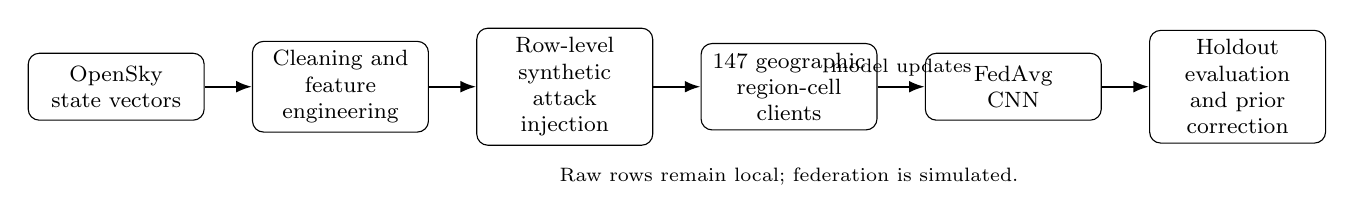
\begin{tikzpicture}[node distance=0.5cm and 0.6cm,box/.style={draw,rounded corners,align=center,text width=2.0cm,minimum height=0.85cm,font=\footnotesize},arr/.style={-{Latex[length=2mm]},thick}]

\node[box] (raw) {OpenSky\\state vectors};\node[box,right=of raw] (clean) {Cleaning and\\feature engineering};\node[box,right=of clean] (inj) {Row-level synthetic\\attack injection};\node[box,right=of inj] (client) {147 geographic\\region-cell clients};\node[box,right=of client] (fed) {FedAvg\\CNN};\node[box,right=of fed] (eval) {Holdout evaluation\\and prior correction};

\draw[arr] (raw)--(clean);\draw[arr] (clean)--(inj);\draw[arr] (inj)--(client);\draw[arr] (client)--node[above,font=\scriptsize]{model updates}(fed);\draw[arr] (fed)--(eval);

\node[below=0.35cm of client,font=\scriptsize] {Raw rows remain local; federation is simulated.};\end{tikzpicture}

\caption{Study pipeline. Centralized LightGBM uses the same capped sample as the federated model.}\label{fig:pipeline}\end{figure*}



\section{The Flooding Artifact}

\subsection{Defect and Correction}

Before correction, three rate features shared a denominator guard that replaced gaps below 1 s with missingness. Flooding duplicates are spaced 0.01--0.5 s apart, so the guard blanked implied speed, speed-consistency delta, vertical-rate-consistency delta, and turn rate together. Filling the resulting missing values with $-1$ created a repeated $(-1,-1,-1,-1)$ token highly correlated with the flooding label. The guard was replaced by a 0.1-s floor, while session breaks remain missing:

\begin{align}
\Delta t_{\rm old}&=\begin{cases}
\Delta t,& |\Delta t|\geq1\text{ s and not a session break},\\
\mathrm{NaN},&\text{otherwise},
\end{cases}\\
\Delta t_{\rm new}&=\begin{cases}
\mathrm{NaN},&\text{session break},\\
\max(\Delta t,0.1),&\text{otherwise}.
\end{cases}
\end{align}
The unfloored inter-arrival feature was unchanged to preserve the short-gap signal.

A flooding group contains one original row and $k$ duplicates, where $k$ is uniform from 2 to 10. Thus, the expected fraction of group rows bearing the old token is
\begin{equation}\frac{\mathbb{E}[k]}{1+\mathbb{E}[k]}=\frac{6}{7}\approx0.857.\end{equation}
The measured pre-fix share was 0.8575--0.858. In a controlled ablation on 300 pre-fix holdout rows, replacing only the four sentinel values by scaler means while holding inter-arrival time fixed reduced mean flooding confidence from 0.8922 to 0.0000 and accuracy from 100\% to 0\%. In a natural flooding evaluation set of 1,143,664 rows, token-bearing rows were classified at 99.9\% accuracy; rows without the token had 1.0\% accuracy, with 85.1\% of those predicted benign. \todo{VERIFY: identify this set; it cannot be a subset of the 688,616-row holdout}
\begin{table}[t]\caption{Rows with Four Kinematic Features Blank}\label{tab:blank}\centering\footnotesize
\begin{tabular}{lrrl}\toprule Class & Before & After & Cause \\
Flooding & 0.8575 & 0.0002 & Corrected artifact \\
Replay & 0.22 & 0.145 & Partly structural \\
Ghost aircraft & 0.98 & 0.98 & Structural masking \\
\bottomrule\end{tabular}\end{table}
All five labeled days were checked after correction; flooding's blank share was 0.0002. The ablation results above are pre-fix; all performance results in Section VIII use the corrected pipeline. The ghost pattern is unaffected: a fabricated address usually makes a one-row aircraft block whose first row is masked. Thus the near-perfect ghost recall reflects the injection construction, not behavioral detection.

\subsection{Remaining Leakage Routes}
Benign rows with implied speed above 400 m/s are filtered while attack rows at the same speed remain, making \texttt{is\_physically\_implausible} a near one-sided attack indicator; its LightGBM gain is 1.4\%. The velocity-spoof vertical-rate boost floor exceeds the 2.5-m/s climb threshold, making the post-injection climb flag near-deterministic; its gain is 2.7\%. Dataset-global \texttt{track\_message\_count} depends on later rows within a two-file chunk and carries 16.8\% gain. Ghost detection is structurally exposed through first-row missingness and address-derived count: recall is 99.98\% and 0.98 of ghost rows retain the blank pattern after the fix. The related LightGBM signals, implied speed and track-message count, carry 18.2\% and 16.8\% of gain, respectively. \texttt{squawk\_changed} may conflate changes, missing values, and first rows, pending verification; its gain is 0.2\%. \todo{VERIFY: empirically confirm squawk\_changed null and first-row behavior}

Low feature importance does not prove absence of leakage because correlated features can substitute. The hand-designed validity flags \texttt{is\_low\_coverage\_region} and \texttt{icao24\_valid\_format} each have 0.0\% gain, but this does not establish that the feature set is leakage-free.

\section{Results}
\subsection{Held-Out-Day Comparison}
Both models are evaluated on the same 688,616-row 2019-02-04 holdout. Centralized LightGBM outperforms the federated CNN at every correction strength. The gap is combined across federation and model family; these runs do not separate the two causes. \cite{ke2017}
\begin{table}[t]\caption{Headline Holdout Results}\label{tab:headline}\centering\footnotesize
\begin{tabular}{llrrrr}\toprule $s$ & Model & Accuracy & FAR & Attack recall & Macro F1 \\
0 & Fed. CNN & 66.4\% & 38.7\% & 86.9\% & 67.3\% \\
0 & LightGBM & 83.7\% & 18.2\% & 95.7\% & 76.5\% \\
0.5 & Fed. CNN & 90.2\% & 8.7\% & 85.2\% & 78.8\% \\
0.5 & LightGBM & 95.0\% & 3.7\% & 94.3\% & 87.8\% \\
1.0 & Fed. CNN & 95.2\% & 0.8\% & 72.9\% & 80.8\% \\
1.0 & LightGBM & 97.3\% & 0.5\% & 92.0\% & 93.9\% \\
\bottomrule\end{tabular}\end{table}

For the CNN, false alarms fall from 38.7\% to 0.8\% between strengths 0 and 1.0, while average attack recall falls from 86.9\% to 72.9\%. The accuracy increase is therefore largely a base-rate effect on a holdout that is 79.32\% benign. At strength 0.5 the CNN has 85.2\% attack recall and 8.7\% false alarms. Across correction strengths, flooding recall remains between 85.49\% and 85.85\%, while replay recall declines from 74.21\% to 71.61\%. Ghost recall remains 99.98\%, but this reflects the structural blank-feature signature. GPS-spoof recall is 81.08\% without correction and 80.75\% at the two corrected settings, whereas its precision rises from 44.49\% to 84.35\% and 84.36\%. These class-wise patterns show why accuracy alone obscures the effect of the prior adjustment.
\begin{figure}[t]\centering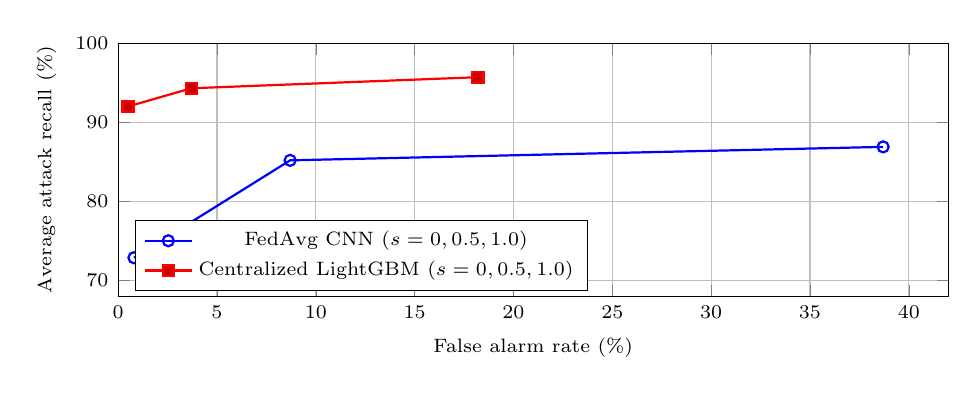
\begin{tikzpicture}\begin{axis}[width=\columnwidth,height=4.8cm,xlabel={False alarm rate (\%)},ylabel={Average attack recall (\%)},xmin=0,xmax=42,ymin=68,ymax=100,grid=both,legend style={font=\scriptsize,at={(0.02,0.02)},anchor=south west},tick label style={font=\scriptsize},label style={font=\scriptsize}]
\addplot+[mark=o,thick] coordinates {(38.7,86.9)(8.7,85.2)(0.8,72.9)};\addlegendentry{FedAvg CNN ($s=0,0.5,1.0$)}
\addplot+[mark=square*,thick] coordinates {(18.2,95.7)(3.7,94.3)(0.5,92.0)};\addlegendentry{Centralized LightGBM ($s=0,0.5,1.0$)}\end{axis}\end{tikzpicture}\caption{False alarm rate versus average attack recall. Points are connected in increasing correction-strength order.}\label{fig:tradeoff}\end{figure}

\subsection{Per-Class Results}
Uncorrected, 194,038 benign rows are predicted as velocity spoofing, or 92\% of all false alarms; velocity-spoof precision is 5.71\%. At full correction its recall falls to 26.12\%, with 8,949 velocity-spoof rows assigned to benign. LightGBM retains 95.0\% velocity-spoof recall at full correction, making this a CNN calibration weakness under the decision rule. Flooding dominates mix-dependent attack metrics because it is the largest synthetic attack class.
\begin{table}[!t]
\caption{Federated CNN Per-Class Recall/Precision (recall / precision, \%)}
\label{tab:perclass}
\centering
\scriptsize
\begin{tabular}{lccc}
\toprule
Class & $s=0$ & $s=0.5$ & $s=1.0$ \\
\midrule
Benign & 61.31 / 97.35 & 91.35 / 97.19 & 99.18 / 95.81 \\
Flooding & 85.49 / 93.96 & 85.85 / 94.79 & 85.85 / 95.82 \\
Ghost aircraft & 99.98 / 97.98 & 99.98 / 98.67 & 99.98 / 99.34 \\
GPS spoof & 81.08 / 44.49 & 80.75 / 84.35 & 80.75 / 84.36 \\
Replay & 74.21 / 70.02 & 72.45 / 75.44 & 71.61 / 86.18 \\
Velocity spoof & 93.63 / 5.71 & 86.76 / 20.28 & 26.12 / 58.18 \\
\bottomrule
\end{tabular}
\end{table}
\begin{figure}[t]\centering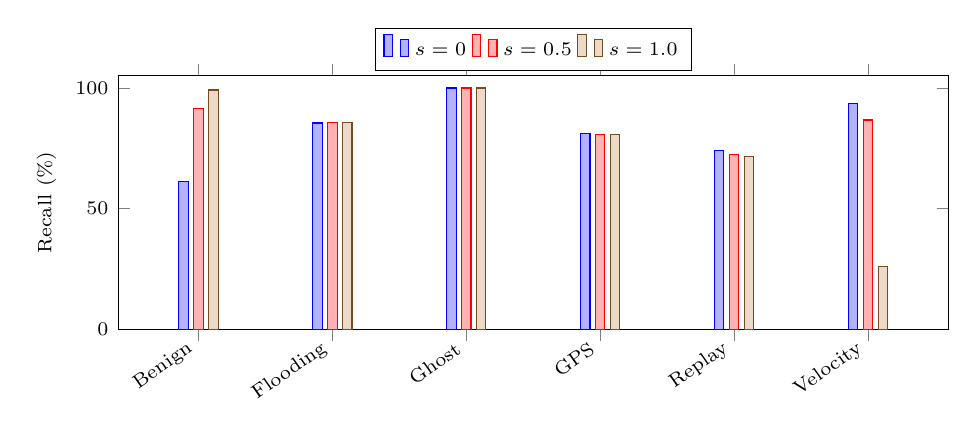
\begin{tikzpicture}\begin{axis}[ybar,bar width=3.4pt,width=\columnwidth,height=4.8cm,ylabel={Recall (\%)},ymin=0,ymax=105,symbolic x coords={Benign,Flooding,Ghost,GPS,Replay,Velocity},xtick=data,xticklabel style={rotate=35,anchor=east,font=\scriptsize},tick label style={font=\scriptsize},label style={font=\scriptsize},legend style={font=\scriptsize,at={(0.5,1.02)},anchor=south,legend columns=3},enlarge x limits=0.12]
\addplot coordinates {(Benign,61.31)(Flooding,85.49)(Ghost,99.98)(GPS,81.08)(Replay,74.21)(Velocity,93.63)};\addlegendentry{$s=0$}
\addplot coordinates {(Benign,91.35)(Flooding,85.85)(Ghost,99.98)(GPS,80.75)(Replay,72.45)(Velocity,86.76)};\addlegendentry{$s=0.5$}
\addplot coordinates {(Benign,99.18)(Flooding,85.85)(Ghost,99.98)(GPS,80.75)(Replay,71.61)(Velocity,26.12)};\addlegendentry{$s=1.0$}\end{axis}\end{tikzpicture}\caption{Federated CNN recall by class at each correction strength.}\label{fig:classrecall}\end{figure}

\subsection{Training, Communication, and Feature Importance}
The best checkpoint is round 46 of 50; pooled accuracy is 0.8283 versus 0.8277 at round 50. Training and test accuracy flatten from about round 40, and the train--test gap ranges from 0.035 to 0.056. The results do not include run-to-run variation, so these training traces should be read as behavior from one seeded run rather than evidence about stability across runs. Per-client local test accuracy ranges from roughly 0.40 to 0.94. The model has 11,334 parameters stored as float32 and a transfer size of 44.3 KB (45,336 bytes). Counting both download and upload, communication totals are $2\times50~\mathrm{rounds}\times147~\mathrm{clients}\times45{,}336~\mathrm{bytes}=666{,}439{,}200~\mathrm{bytes}$ (666.44 MB), or 13.329 MB per round.
\begin{table}[!t]\caption{LightGBM Feature Importance (Gain Share)}\label{tab:importance}\centering\footnotesize
\setlength{\tabcolsep}{4pt}\begin{tabular}{lr|lr}\toprule Feature & Gain & Feature & Gain \\
inter\_arrival\_s & 37.3\% & is\_climbing\_or\_descending & 2.7\% \\
implied\_speed\_mps & 18.2\% & is\_physically\_implausible & 1.4\% \\
track\_message\_count & 16.8\% & region\_avg\_inter\_arrival & 1.1\% \\
vrate\_consistency\_delta & 11.3\% & turn\_rate\_deg\_s & 0.8\% \\
speed\_consistency\_delta & 9.5\% & is\_stale & 0.7\% \\
squawk\_changed & 0.2\% & is\_low\_coverage\_region & 0.0\% \\
 & & icao24\_valid\_format & 0.0\% \\
\bottomrule\end{tabular}\end{table}
The top five features carry 93.1\% of gain; both validity flags have 0.0\% gain. Correlated features may substitute, so low gain does not rule out leakage.

\section{Limitations}
All reported results use a single random seed, so no run-to-run variance is available. The federated CNN is compared with centralized LightGBM; this gap is combined across federation and model family, not a measured cost of privacy. No centralized CNN or federated tree baseline was evaluated. Benign traffic is real but all attacks are synthetic, independently selected per row rather than generated as coherent aircraft-level episodes. No real attack data validate the detector, and an adaptive attacker aware of the features could evade the rules. The injection rate is about 2\%, above the 0.05\% attributed to Li \emph{et al.}; the citation and rate need verification, and the model has not seen realistic prevalence. Replay uses a sampled time shift rather than the fixed delay attributed to Li; flooding duplicates at sub-second offsets and is not claimed equivalent to a time-window denial-of-service pattern. \todo{VERIFY: confirm Li et al. parameter values and flooding comparison}

Only one geographic partition of the sampled data was evaluated. The five source days are winter Mondays from 2019-01-07 through 2019-02-04. The holdout is one day, uses the same attack generator, and is not aircraft-disjoint from training; day- and schedule-specific effects may carry across the split. The cap and injection procedure are also reused across the split, so the holdout tests a later day under the same synthetic labeling rules rather than an independently designed threat model. OpenSky coverage gaps and data quality vary geographically. Ghost-aircraft performance is structural: the synthetic rows leave kinematic fields blank and usually have a one-row address count, so near-perfect recall is not behavioral validation.

Federation is simulated in one process with all 147 clients participating every round, without dropout, stragglers, or network failures. There is no differential privacy or secure aggregation; only raw-row locality is claimed. The pooled scaler, pooled class weights, and globally capped-sample partition are centralizations a deployment could not perform. Checkpoint selection and pooled test accuracy use the same split, making the latter mildly optimistic; held-out-day scores are separate. Non-IID client data and the listed feature-leakage routes also limit interpretation. Latency and real-time operation were not measured, so no operational-readiness claim is supported; the intended scope is situational awareness and threat intelligence, not real-time TCAS replacement.

\section{Conclusion and Future Work}
This paper reports a geographic FedAvg simulation using real OpenSky observations and five row-level synthetic attack types. A flooding-related feature artifact was explained analytically, confirmed by targeted ablation, and removed by flooring the rate denominator. Centralized LightGBM outperformed the federated CNN on a single held-out day at each correction strength. The combined comparison does not isolate federation. Class-prior correction reduced false alarms but also reduced average attack recall, particularly because of velocity-spoof calibration.

Future work should include centralized and local-only baselines of the same model, FedProx and personalization, multiple seeds, aircraft-disjoint splits, coherent episode-level attacks, causal features, per-class prior correction, ratio-based correction using deployment and training priors, and training under realistic prevalence. Further evaluation on additional days and operationally representative feeds is needed before conclusions about deployment or privacy-performance tradeoffs.

\section*{Reproducibility}
Code and data access details will be made available at \todo{REPOSITORY: add code and data repository link}. Reproducibility commands and local paths are omitted.

\begin{thebibliography}{00}
\bibitem{mcmahan2017} B. McMahan, E. Moore, D. Ramage, S. Hampson, and B. Aguera y Arcas, ``Communication-Efficient Learning of Deep Networks from Decentralized Data,'' in \emph{Proceedings of the 20th International Conference on Artificial Intelligence and Statistics}, vol. 54, pp. 1273--1282, 2017.
\bibitem{ying2019} Ying \emph{et al.}, ``Detecting ADS-B Spoofing Attacks using Deep Neural Networks,'' arXiv:1904.09969, 2019.
\bibitem{ngamboe2025} Ngamboe \emph{et al.}, ``New Machine Learning Approaches for Intrusion Detection in ADS-B,'' arXiv:2510.08333, 2025.
\bibitem{li2020} \todo{VERIFY authors against doi:10.1049/iet-ifs.2018.5635}, ``\todo{VERIFY title against doi:10.1049/iet-ifs.2018.5635},'' \emph{IET Information Security}, vol. 14, no. 5, pp. \todo{VERIFY pages against doi:10.1049/iet-ifs.2018.5635}, 2020, doi:10.1049/iet-ifs.2018.5635.
\bibitem{ke2017} G. Ke \emph{et al.}, ``LightGBM: A Highly Efficient Gradient Boosting Decision Tree,'' in \emph{Advances in Neural Information Processing Systems}, vol. 30, 2017.
\end{thebibliography}
\end{document}